\section{Projektmanagement - Begriff}
Für das gemeinsame Verständnis des Begriffes ``Projektmanagement'' wird zuerst
eine Definition des Wortes gemacht. Diese Arbeit lehnt sich an diese 
Begriffsdefinition an. Danach wird näher auf den Aufbau eines
Projektablaufes eingegangen.

Im Rahmen eines Projektmanagement werden die diversen Aufgaben ganzheitlich in
einem Projekt eingebettet und unter Berücksichtigung der Parameter Kosten, Termine
und Qualität geplant und durchgeführt.\footnote{\citealp*[Vgl.][S. 9]{burghardt2007einfuehrung}}
Die Stiftung für Forschung und Beratung am Betriebswissenschaftlichen Institut 
(BWI) der ETH Zürich definiert den Begriff Projektmanagement wie folgt:

\begin{quote}
``Projektmanagement wird als Überbegriff aller planenden, überwachenden,
koordinierenden und steuernden Massnahmen verstanden, die für die Um- oder
Neugestaltung von Systemen (resp. Problemlösungen) erforderlich sind.''\footnote{\citealp*[S. 1.1]{stiftung1998projekt}}
\end{quote}

\section{Projektablauf}
Der Projektablauf gehört zu den Methoden und Techniken der Organisation. Als
Projekt bezeichnet man ein Vorhaben, das einmalig ist und einen definierten
Start- und Endtermin hat. Im Projektablauf regelt man die Ablauforganisation
eines Projektes, also welche Aufgaben wann zu erledigen sind.\footnote{\citealp*[Vgl.][S. 136]{schmidt2002einfuehrung}}
Das Projektmanagement mit dem Projektablauf als Methode umfasst alle Aktivitäten,
die für eine vollständige Abwicklung eines Projektes erforderlich sind.\footnote{\citealp*[Vgl.][S. 11]{burghardt2007einfuehrung}}

Ein Projektablauf unterteilt man in vier Hauptabschnitte, die in der Abbildung \ref{pic:01_hauptabschnitte}
dargestellten sind.

\clearpage

\begin{figure}[htbp]
\begin{center}

\includegraphics[width=0.85\textwidth,angle=0]{./bilder/theorie/01_hauptabschnitte.pdf}
\caption[Vier Hauptabschnitte eines Projektablaufes]{Vier Hauptabschnitte eines Projektablaufes\footnotemark}
\label{pic:01_hauptabschnitte}
\end{center}
\end{figure}
\footnotetext{Eigene Darstellung in Anlehnung an \citealp*[Bild 1.2]{burghardt2007einfuehrung}}

\subsection{Projektdefinition}
Die Projektdefinition besteht aus der eigentlichen Gründung eines Projektes,
der Definition des Projektziels und die Organisation des Projektes.

Zu Beginn eines Projektes steht der Projektantrag. Er beinhaltetet alle relevanten
Informationen wie eine Aufgabenbeschreibung und Termine. Wird der Projektantrag
angenommen, wandelt sich der Antrag in einen Projektauftrag um.\footnote{\citealp*[Vgl.][S. 13]{burghardt2007einfuehrung}}
Als nächstes muss ein eindeutiges und vollständiges Projektziel definiert werden.
Dies geschieht meist zusammen mit dem Auftraggeber anhand eines Anforderungskatalogs
oder Pflichtenhefts.

Es empfiehlt sich eine Problemfeldanalyse und eine Wirtschaftlichkeitsbetrachtung
zu machen. Ohne genauere Kenntnisse zur Wirtschaftlichkeit eines Projektes sollte
keines begonnen werden.\footnote{\citealp*[Vgl.][S. 45]{burghardt2007einfuehrung}}
Unter einer Problemfeldanalyse versteht man eine klare Definition des eigentlichen
Problems. Wobei das Problem eher als Herausforderung zu betrachten ist. Man
stellt sich dabei folgende Fragen:

\begin{itemize}
    \item Was ist das Problem bzw. die Herausforderung?
    \item Wer sind die Betroffenen und die Beteiligten?
    \item Was sind deren wichtigste Ziele?
\end{itemize}

Bei der Überprüfung der Wirtschaftlichkeit eines Projektes kann dies im Sinne
des Endproduktes oder des Auftrages geschehen. Im Ersteren versucht man zu
errechnen, ob das Endprodukt einen wirtschaftlichen Nutzen für den Auftraggeber
darstellt. Dies sollte der Auftraggeber normalerweise schon selbst vorgenommen
haben. Für die Projektleitung steht schlussendlich der wirtschaftliche Nutzen
des Auftrages für die eigene Unternehmung im Vordergrund. Kann der Auftrag so
offeriert und durchgeführt werden, dass das Projekt am Ende profitabel ist.\footnote{\citealp*[Vgl.][S. 4]{prueter2007multi}}

Ist dies zutreffend, müssen die organisatorischen Voraussetzungen für das Projekt geschaffen werden,
indem der Projektleiter ernannt und eine passende Projektorganisation gewählt wird.
Die Definition einer Projektorganisation lautet nach DIN 69901:

\begin{quote}
``Gesamtheit der Organisationseinheiten und der aufbau- und ablauforganisatorischen
Regelungen zur Abwicklung eines bestimmten Projektes.''\footnote{Vgl. DIN 69901}
\end{quote}

Je nach Bereichsüberschreitung innerhalb des Unternehmens und der einzubindenden
Projektmitarbeiter sowie der Bedeutung und der Grösse des Projektes kann zwischen
fünf Formen von Projektorganisationen unterschieden werden:\footnote{\citealp*[Vgl.][S. 56]{burghardt2007einfuehrung}}

\begin{itemize}
    \item Reine Projektorganisation
    \item Einfluss-Projektorganisation
    \item Matrix-Projektorganisation
    \item Auftrags-Projektorganisation
    \item Projektmanagement in der Linie
\end{itemize}

In der reinen Projektorganisation wir in der bestehenden Unternehmensstruktur
eine zusätzliche Stelle für das Projekt geschaffen und alle beteiligten 
Projektmitarbeiter unter einem Projektleiter, der die Linienautorität hat, 
zusammengefasst.\footnote{\citealp*[Vgl.][S. 56]{burghardt2007einfuehrung}}
In der Grafik \ref{pic:05_projektorganisationen_reine} ist 
ein Beispiel einer reinen Projektorganisation abgebildet.

\begin{figure}[htbp]
\begin{center}
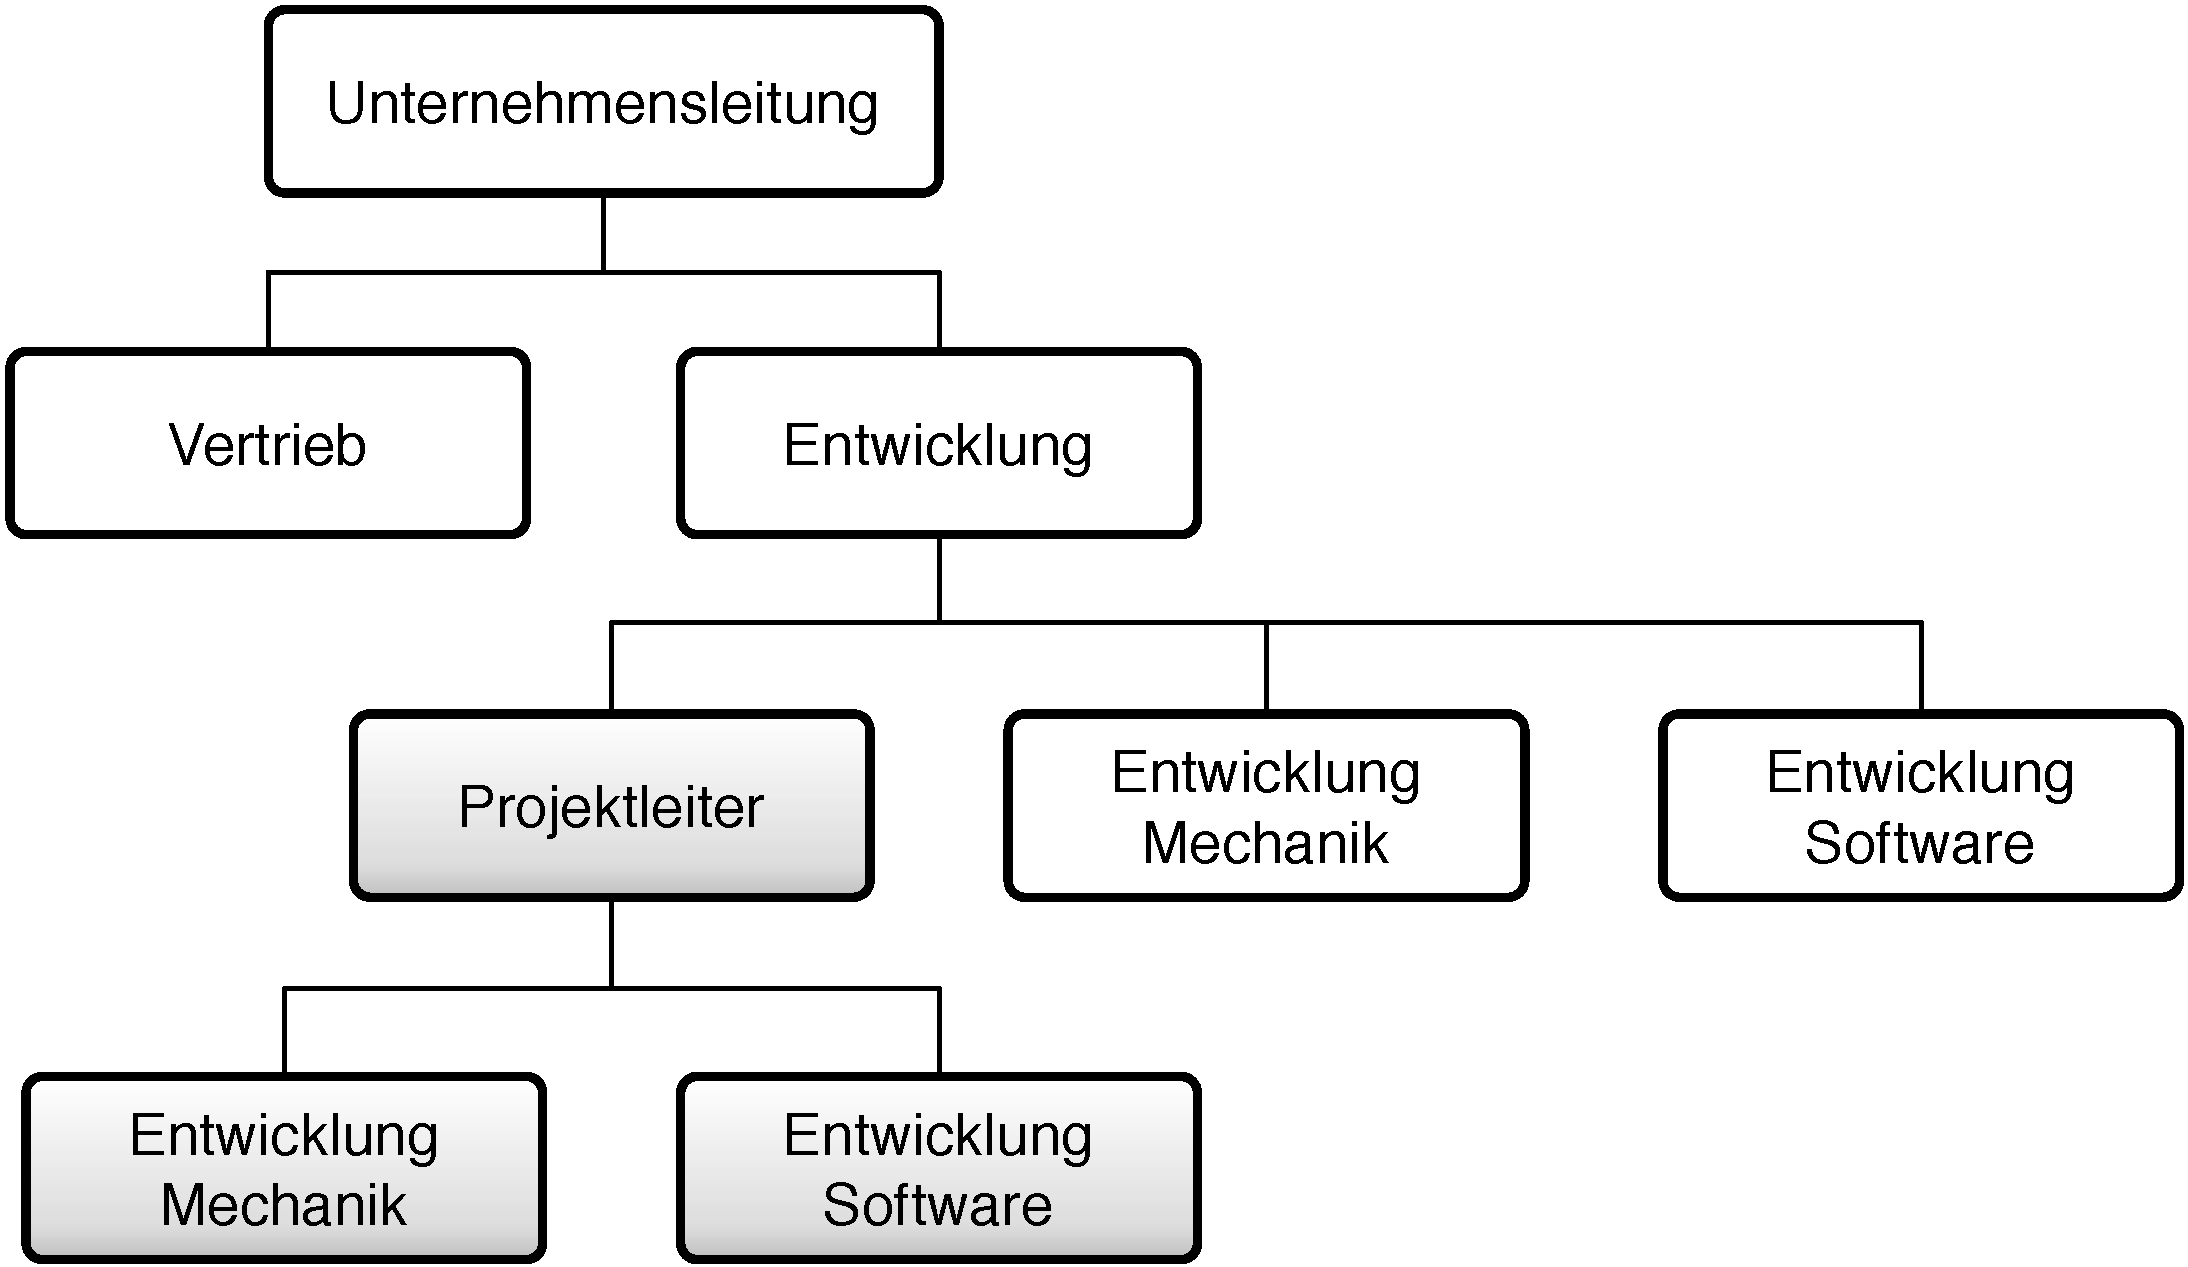
\includegraphics[width=0.5\textwidth,angle=0]{./bilder/theorie/05_projektorganisationen_reine.pdf}
\caption[Reine Projektorganisation]{Reine Projektorganisation\footnotemark}
\label{pic:05_projektorganisationen_reine}
\end{center}
\end{figure}
\footnotetext{Eigene Darstellung in Anlehnung an \citealp*[Bild 2.9]{burghardt2007einfuehrung}}

In einer Einlfuss-Projektorganisation gibt es anstelle einem Projektleiter
einen Projektkoordinator, der als Stabsstelle eingefügt. Er hat jedoch kaum
Kompetenzen und kann nur koordinierend und lenkend wirken.\footnote{\citealp*[Vgl.][S. 57]{burghardt2007einfuehrung}}
In der Grafik \ref{pic:05_projektorganisationen_einfluss}
ist ein Beispiel einer Einfluss-Projektorganisation abgebildet.

\clearpage

\begin{figure}[htbp]
\begin{center}
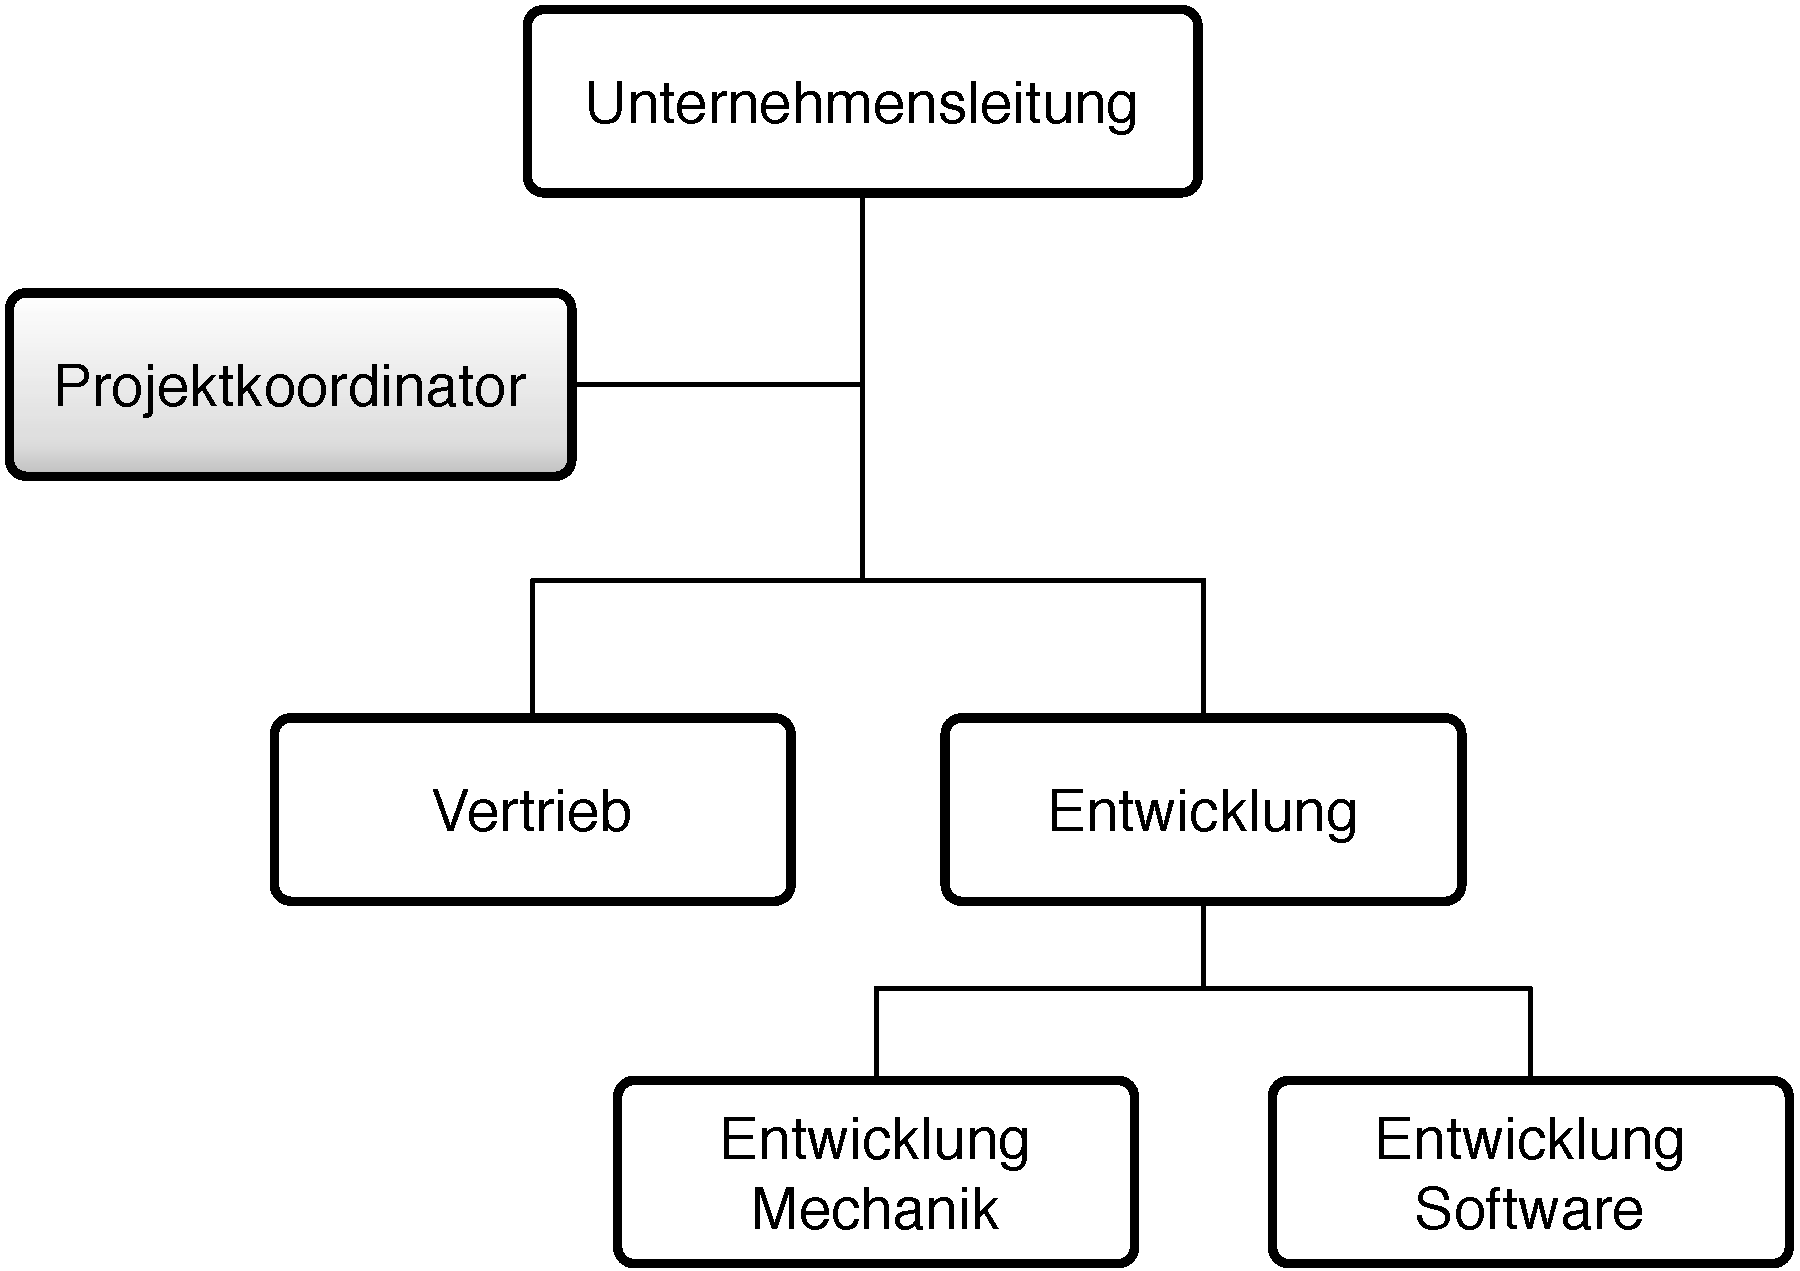
\includegraphics[width=0.45\textwidth,angle=0]{./bilder/theorie/05_projektorganisationen_einfluss.pdf}
\caption[Einfluss-Projektorganisation]{Einfluss-Projektorganisation\footnotemark}
\label{pic:05_projektorganisationen_einfluss}
\end{center}
\end{figure}
\footnotetext{Eigene Darstellung in Anlehnung an \citealp*[Bild 2.10]{burghardt2007einfuehrung}}

In der Matrix-Projektorganisation trägt der Projektleiter zwar die ganze Verantwortung
des Projektes, hat aber nicht die ganze Weisungsbefugnis für alle beteiligten Mitarbeiter.
Die fachliche Weisungsbefugnis unterliegt zwar dem Projektleiter, die disziplinarische
bleibt jedoch weiterhin beim direkten Vorgesetzten in der Linienorganisation.\footnote{\citealp*[Vgl.][S. 58]{burghardt2007einfuehrung}}
In der Grafik \ref{pic:05_projektorganisationen_matrix} ist ein Beispiel einer 
Marix-Projektorganisation abgebildet.

\begin{figure}[htbp]
\begin{center}
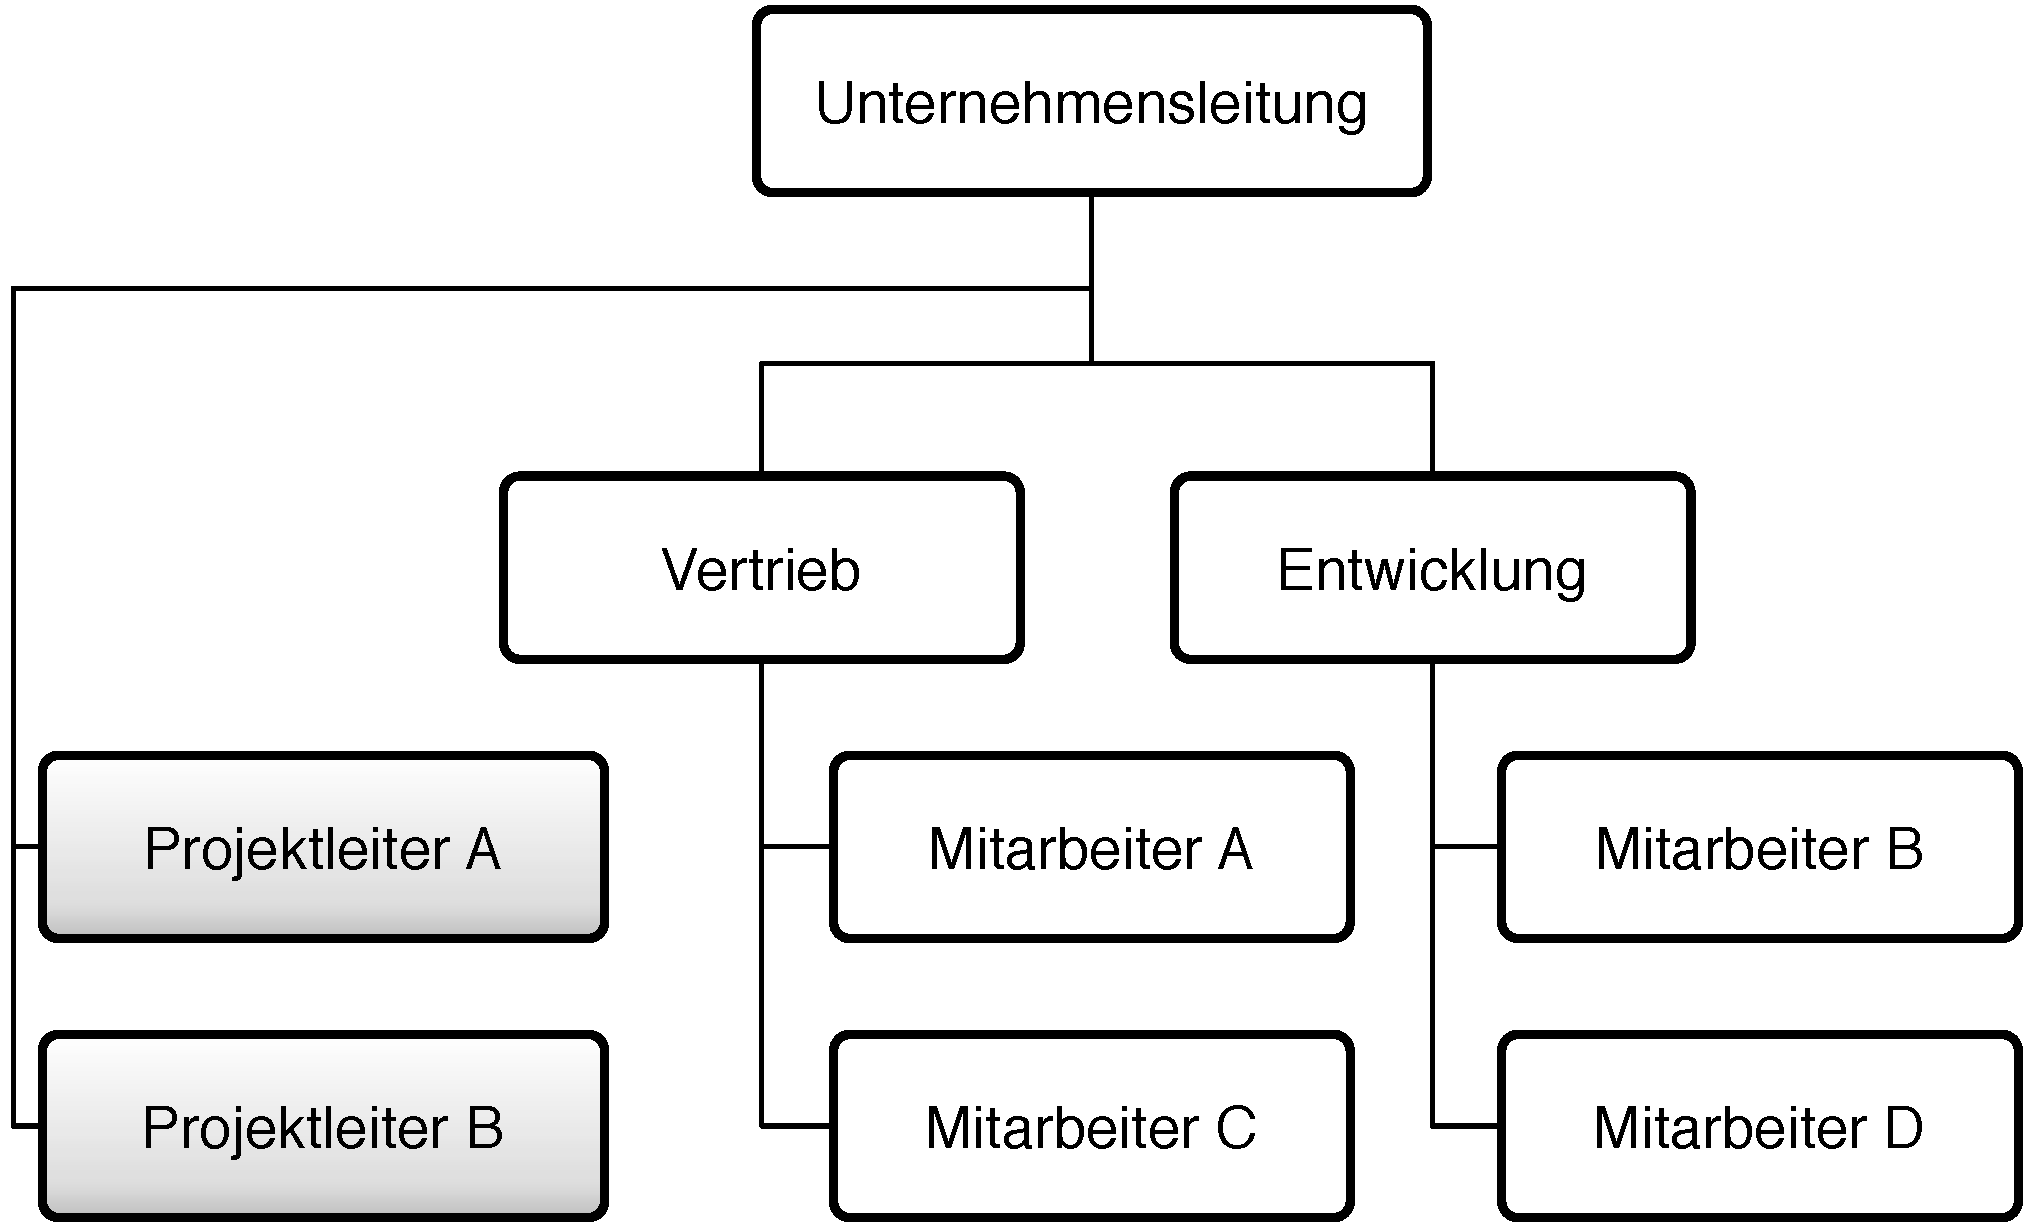
\includegraphics[width=0.5\textwidth,angle=0]{./bilder/theorie/05_projektorganisationen_matrix.pdf}
\caption[Matrix-Projektorganisation]{Matrix-Projektorganisation\footnotemark}
\label{pic:05_projektorganisationen_matrix}
\end{center}
\end{figure}
\footnotetext{Eigene Darstellung in Anlehnung an \citealp*[Bild 2.11]{burghardt2007einfuehrung}}

Die Auftrags-Projektorganisation ist ebenfalls eine matrixorientierte 
Organisationsform. Bei dieser gibt es aber keine Doppelunterstellung der Mitarbeiter.
Somit ist hier der Projektleiter auch für die fachtechnische Durchführung des
Projektes verantwortlich.\footnote{\citealp*[Vgl.][S. 58]{burghardt2007einfuehrung}}
In der Grafik \ref{pic:05_projektorganisationen_auftrags}
ist ein Beispiel einer Marix-Projektorganisation abgebildet.

\clearpage

\begin{figure}[htbp]
\begin{center}
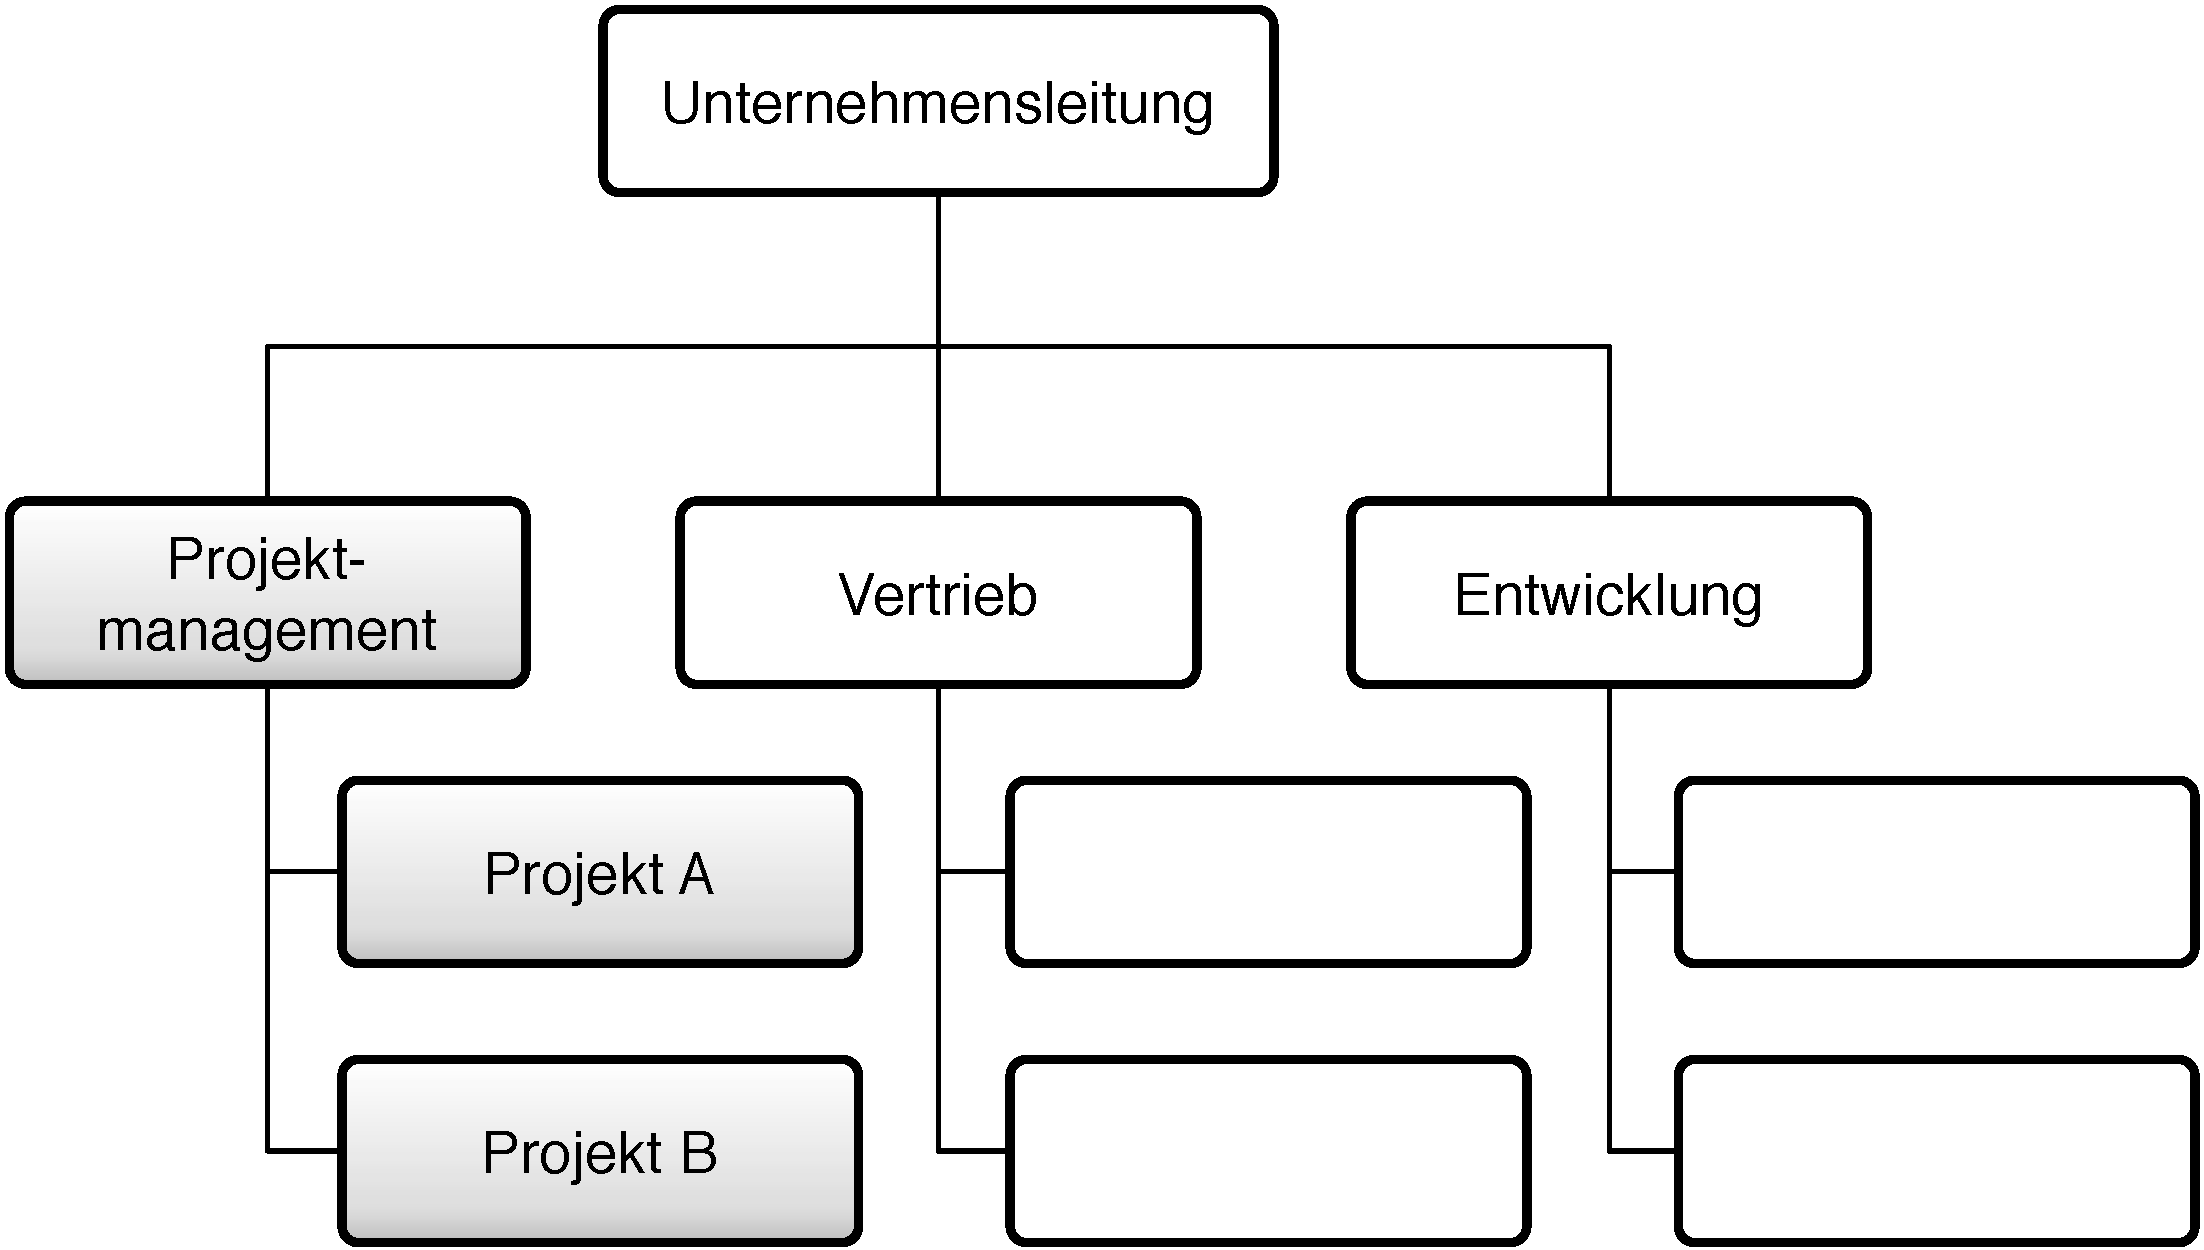
\includegraphics[width=0.55\textwidth,angle=0]{./bilder/theorie/05_projektorganisationen_auftrags.pdf}
\caption[Auftrags-Projektorganisation]{Auftrags-Projektorganisation\footnotemark}
\label{pic:05_projektorganisationen_auftrags}
\end{center}
\end{figure}
\footnotetext{Eigene Darstellung in Anlehnung an \citealp*[Bild 2.12]{burghardt2007einfuehrung}}

Die Durchführung eines Projektes erfordert nicht immer ein Einrichten einer eigenen
Projektorganisation. Beim Projektmanagement über die Linie wird ebenfalls ein
Projektleiter ernannt, der dann meist eine Art Gruppenführer-Funktion einnimmt,
ähnlich wie bei der Einfluss-Projektorganisation.

\subsection{Projektplanung}
In der Projektplanung definiert man die Strukturplanung, eine Aufwandschätzung,
die Arbeits- und Kostenplanung sowie das Risikomanagement.

In der Strukturplanung wird das Vorhaben technisch, aufgabengemäss und kaufmännisch
anhand den Anforderungen strukturiert. Auf den sich ergebenden Strukturen bauen
alle weiteren Planungsschritte auf. Danach werden daraus die einzelnen Aufgabenpakete
abgeleitet, für die dann eine Aufwandsschätzung durchzuführen ist.\footnote{\citealp*[Vgl.][S. 14]{burghardt2007einfuehrung}}
Wenn möglich sollten zur Schätzung nebst dem eigenen Erfahrungspotential auch
Erfahrungen von Experten zum Thema herangezogen werden.

Ein allgemeines Schema zur Vorgehensweise zum Sammeln von Erfahrungswerten zur 
Aufwandsschätzung ist in der Grafik \ref{pic:02_schema_aufwandsschaetzung}
abgebildet.

\clearpage

\begin{figure}[htbp]
\begin{center}
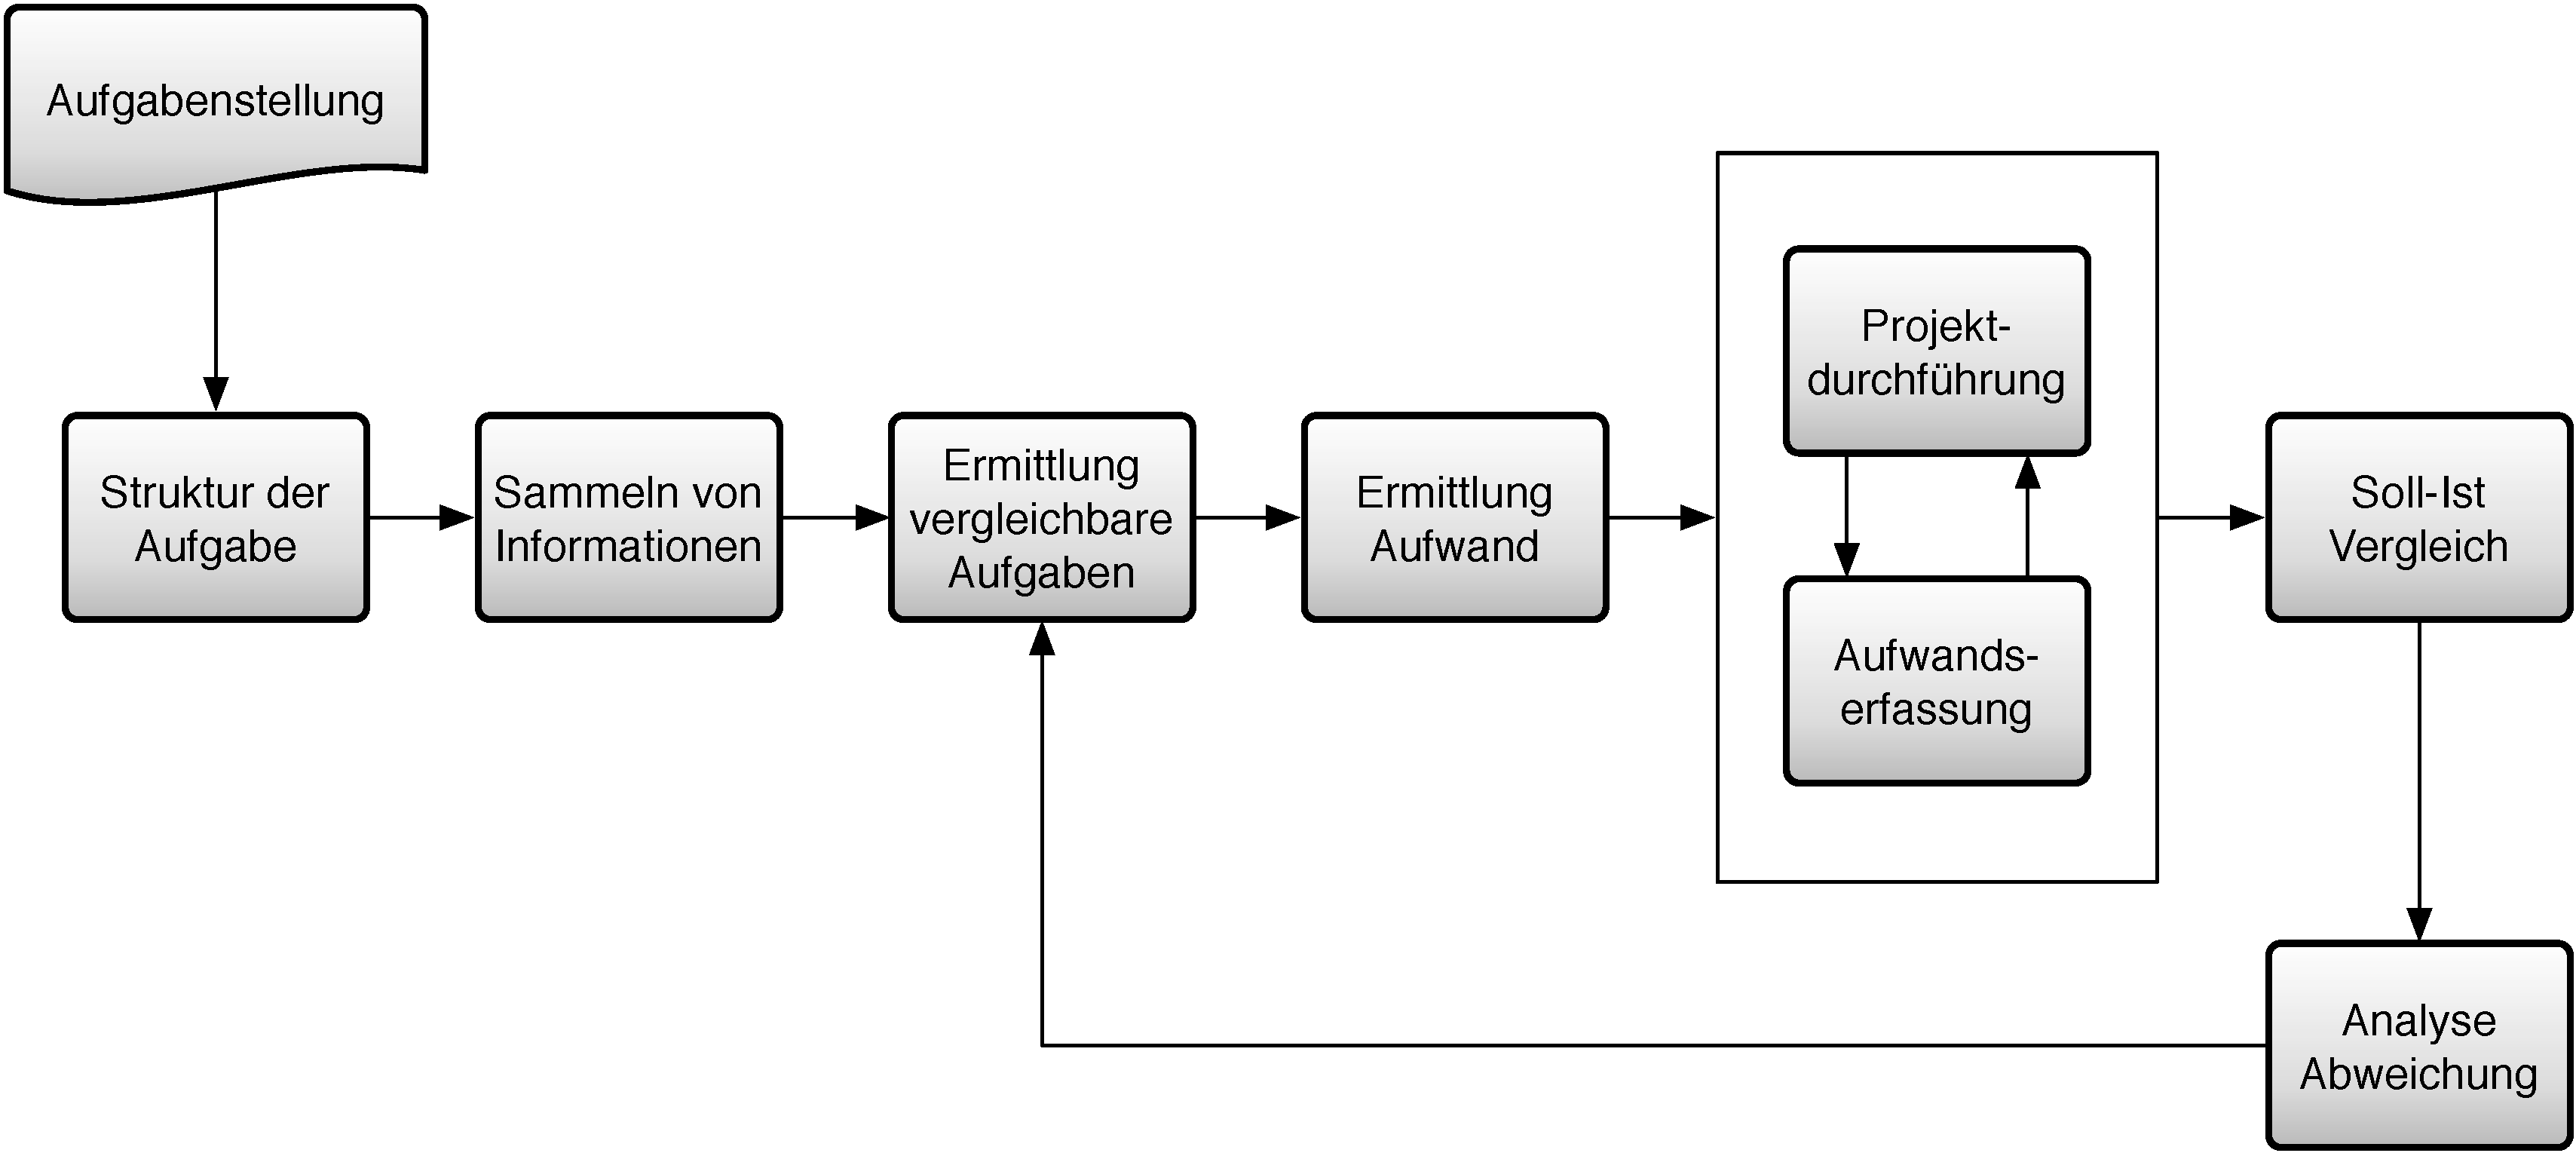
\includegraphics[width=0.75\textwidth,angle=0]{./bilder/theorie/02_schema_aufwandsschaetzung.pdf}
\caption[Sammeln von Erfahrungswerten zur Aufwandsschätzung]{Sammeln von Erfahrungswerten zur Aufwandsschätzung\footnotemark}
\label{pic:02_schema_aufwandsschaetzung}
\end{center}
\end{figure}
\footnotetext{Eigene Darstellung des Schemas in Anlehnung an \citealp*[S. 112]{litke2007projektmanagement}}

Es gibt diverse Aufwandsschätzungsverfahren die genutzt werden können. Die Methoden unterscheiden
sich beim Schätzverfahren und können zum Beispiel nach folgender Klassifikation 
erfolgen:\footnote{Vgl. \citealp*{noth1986aufwandschaetzung} und \citealp*{knoell1991aufwandsschaetzung}}

\begin{itemize}
    \item Anzahl der Phasen, die abgedeckt werden, zum Beispiel:
    \begin{itemize}
        \item Einzelaktivitäten
        \item Programmierung
        \item Detailentwurf und Programmierung
        \item Gesamter Entwicklungsprozess
    \end{itemize}
    \item Theoretische oder praktische Absicherung, zum Beispiel:
    \begin{itemize}
        \item Unternehmensspezifische Verfahren
        \item Unternehmensunabhängige Praxisverfahren
        \item Wissenschaftlich fundierte Verfahren
    \end{itemize}
    \item Verwendungszweck, zum Beispiel:
    \begin{itemize}
        \item Kosten/Nutzenanalyse zur Kalkulation der Kosten
        \item Kapazitäts- und Terminplanung zur Ermittlung von Plangrössen
    \end{itemize}
\end{itemize}

Anhand den Ergebnissen aus der Aufwandsschätzung werden nun die einzelnen
Arbeitspakete bzw. Teilaufgaben in eine Arbeitsplanung übernommen. Oft empfiehlt
es sich hier einen Netzplan zur Erstellung der Aufgaben- und Terminplanung
anzufertigen. ``Die Netzplantechnik ist trotz aller Kritik eines der 
leistungsfähigsten Projektmanagement-Hilfsmittel, wenn sie richtig eingesetzt wird.''
\footnote{\citealp*[S. 14]{burghardt2007einfuehrung}}

\begin{figure}[htbp]
\begin{center}
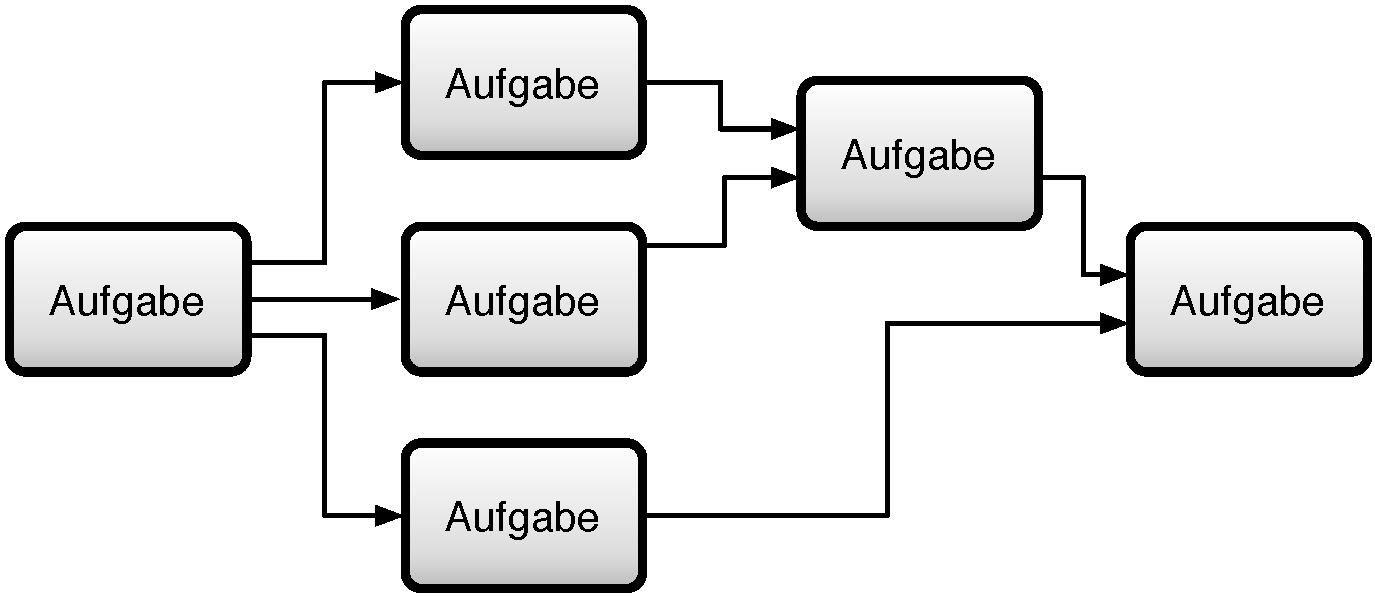
\includegraphics[width=0.5\textwidth,angle=0]{./bilder/theorie/03_darstellung_netzplan.pdf}
\caption[Konzeptionelle Darstellung eines determinisitischen Netzplanes]{Konzeptionelle 
    Darstellung eines determinisitischen Netzplanes\footnotemark}
\label{pic:03_darstellung_netzplan}
\end{center}
\end{figure}
\footnotetext{Eigene Darstellung des Schemas in Anlehnung an \citealp*[Bild 3.17]{burghardt2007einfuehrung}}

% http://books.google.de/books?id=m54LKbnCIoYC&pg=PA155&dq=Netzplantechnik&hl=de&ei=Qai-Tf2dNsmDOqL12dsF&sa=X&oi=book_result&ct=result&resnum=9&ved=0CHYQ6AEwCA#v=onepage&q=Netzplantechnik&f=false

\subsection{Projektkontrolle}
An erster Stelle der Projektkontrolle steht der Plan/Ist-Vergleich der vorgegebenen
Projektparameter. Durch einen laufenden Vergleich im Rahmen der Projektkontrolle
erreicht man, dass Abweichungen frühzeitig erkannt werden. Diese Abweichungen
führen zu ``geeigneten'' Massnahmen, die rechtzeitig ergriffen werden können.
Die Projektkontrolle umfasst im ganzen die Termin-, Aufwands-, Kosten-, 
und Sachfortschrittskontrolle, Qualitätssicherung, Projektdokumentation und
das Personalmanagement.\footnote{\citealp*[Vgl.][S. 15]{burghardt2007einfuehrung}}

Die Terminkontrolle wird in der Praxis so umgesetzt, dass die Einhaltung
und Erreichung der gesetzten Meilensteine kontrolliert wird. Wenn ein 
Meilenstein nicht eingehalten werden kann, muss kontrolliert werden, ob die
weiteren davon betroffen sind. Häufig ist das der Fall und die Termine
müssen angepasst und neu gewählt werden. Hierbei ist es wichtig, den Auftraggeber
über die Veränderungen zu informieren.

Die Aufwands- und Kostenkontrolle wird in der Praxis meist durch die Kontrolle
der rapportierten Stunden durchgeführt. Man sollte in beiden Fällen, also der
Termin- und Aufwandskontrolle, eine Trendanalyse erstellen, um eine mögliche
Entwicklung daraus abzuleiten.

\clearpage

In der Praxis werden immer wieder folgende, in der Grafik \ref{pic:06_trendanalyse}
abgebildeten, sechs typische Kurvenverläufe beobachtet.\footnote{\citealp*[Vgl.][S. 177 und S. 194]{burghardt2007einfuehrung}}

\begin{figure}[htbp]
\begin{center}
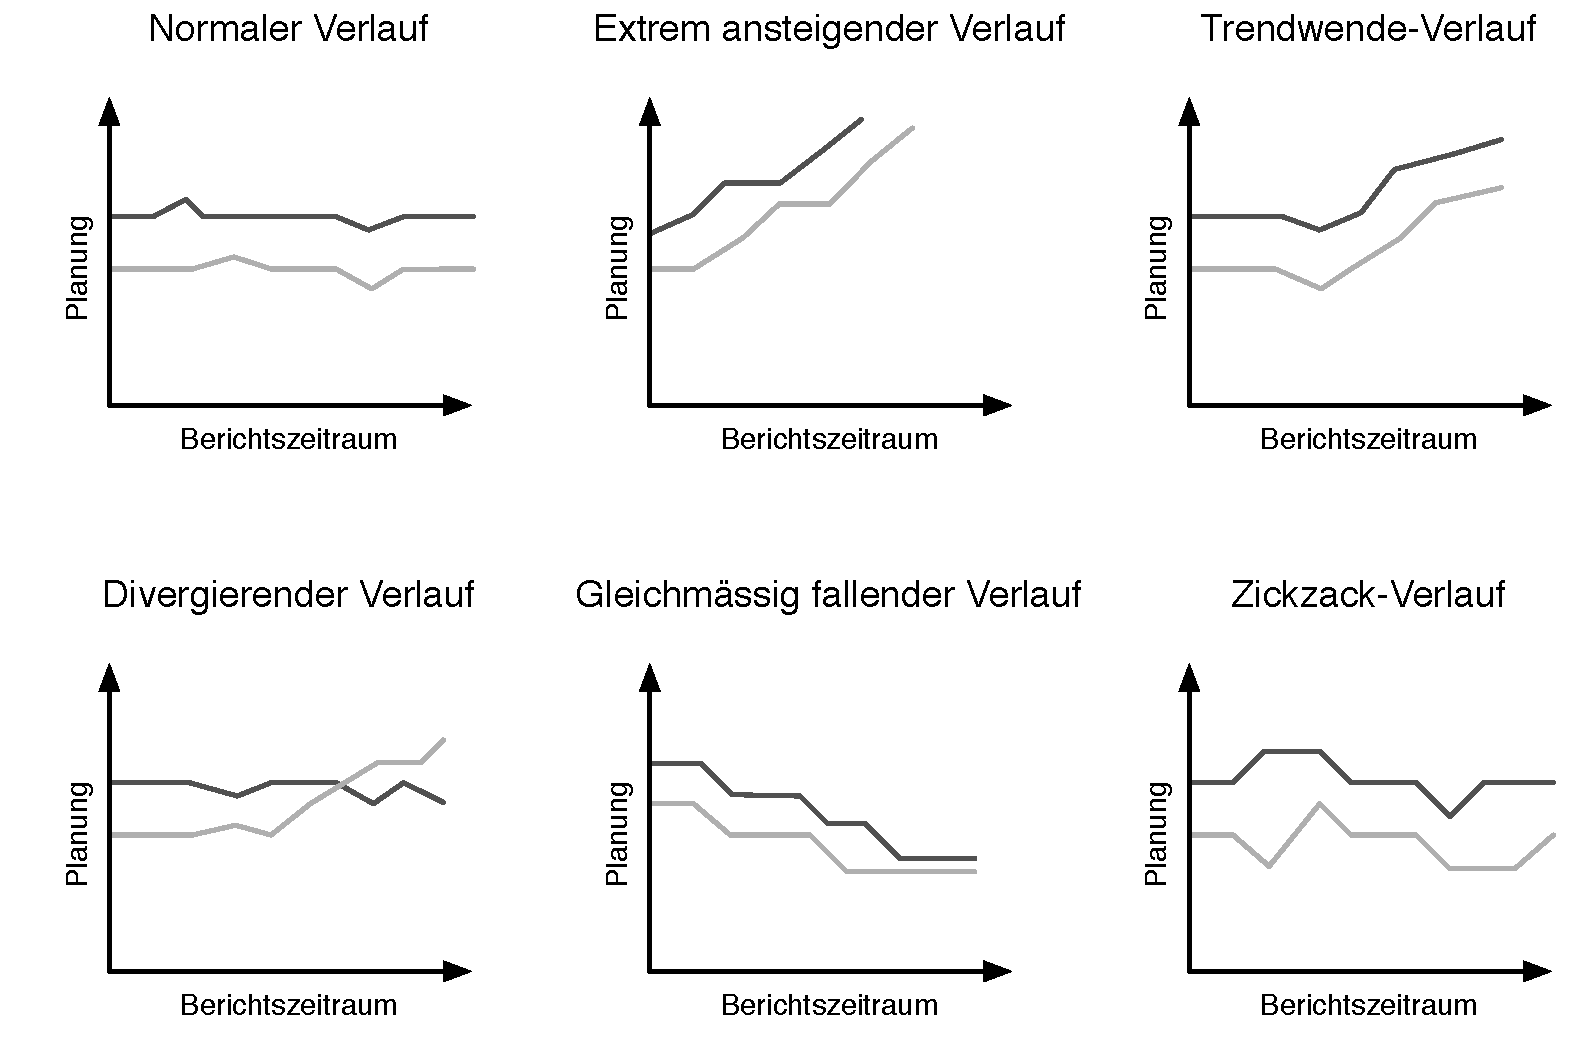
\includegraphics[width=0.8\textwidth,angle=0]{./bilder/theorie/06_trendanalyse.pdf}
\caption[Typische Kurvenverläufe bei Trendanalysen]{Typische Kurvenverläufe bei Trendanalysen\footnotemark}
\label{pic:06_trendanalyse}
\end{center}
\end{figure}
\footnotetext{Eigene Darstellung des Schemas in Anlehnung an \citealp*[Bild 4.4 und 4.13]{burghardt2007einfuehrung}}

\begin{description}
    \item [Normaler Verlauf] Hier sind geringe Termin- und Kostenverschiebungen 
    ablesbar. Mit hoher Wahrscheinlichkeit kann der Gesamttermin und das Budget 
    eingehalten werden.

    \item [Extrem ansteigender Verlauf] Hier wurde anscheinend laufend zu optimistisch geplant 
    und budgetiert. Der Endtermin wird sich mit hoher Wahrscheinlichkeit erheblich 
    verschieben und das Budget wird nicht eingehalten werden können.

    \item [Trendewende-Verlauf] Hier wurden möglicherweise die geplanten Termine 
    und Budgets künstlich eingehalten und die ``Probleme'' nach hinten verschoben. 
    Gegen Ende zeichnet sich eine erhebliche Veränderung ab. Ein rechtzeitiger 
    korrigierender Eingriff wurde dadurch verhindert.

    \item [Divergierender Verlauf] Gehen die Kurven auseinander, kann man ebenfalls 
    von einer falschen Rapportierung ausgehen. Man sollte die Trendanalyse im 
    Nachhinein ganz überarbeiten und korrigieren.
    
    \item [Gleichmässig fallender Verlauf] Hier wurde anscheinend mit einem sehr 
    grossen Sicherheitspuffer geplant. In so einem Fall ist es wichtig, seine
    Aufwandsschätzung am Ende des Projektes korrigiert in die Erfahrung einfliessen
    zu lassen, damit man in Zukunft genauer plant.
    
    \item [Zickzack-Verlauf] Ein solcher Verlauf deutet auf eine grosse
    Unsicherheit bezüglich des Fortschrittes hin. Mit grosser Wahrscheinlichkeit
    wird der Endtermin auch hier nicht eingehalten werden können.
\end{description}

Die Sachfortschrittskontrolle ist eine der wichtigsten Kontrollaufgaben für
den Projektleiter. Es ist zuggleich aber auch die schwierigste, da oft keine
unmittelbare Messgrössen vorhanden sind.
Die Kernfragen, die man sich in der Sachfortschrittskontrolle stellt, sind folgenden:\footnote{\citealp*[Vgl.][S. 134]{jenny2009projektmanagement}}

\begin{itemize}
    \item Wie verhält sich der Projektaufwand zu den erbrachten Leistungen?
    \item Wie hoch ist der Zielerreichungsgrad der definierten Projektziele?
\end{itemize}

Es wird empfohlen, während der Projektdurchführung mehrmals eine Restaufwands-
und Restzeitschätzung vorzunehmen und die Trendanalysen zu aktualisieren.\footnote{\citealp*[Vgl.][S. 16]{burghardt2007einfuehrung}}

Bei der Projektdokumentation handelt es sich um die vollständigen Informationen
über das zu entwickelnde Produkt. Es empfiehlt sich eine Projektakte mit einer
vorgegebenen Ordnung aufzubauen und eine Art Projekttagebuch zu führen, dessen
Inhalt an keine Ordnungssystematik gebunden ist. Die daraus abzulesenden
Informationen werden zur Projektberichterstattung verwendet.

Das Personalmanagement in einem Projekt beinhaltet eine projektkonforme
Personalführung und das Fördern einer positiven Zusammenarbeit in einem
Projektteam. Wichtig ist stets die Akzeptanz der Projektleitung und die 
Motivation der Projektmitarbeiter. Ein gutes Konfliktmanagement spielt
dabei ebenfalls eine wichtige Rolle, damit man auf Konflikte innerhalb des
Projektes frühzeitig reagieren und sie bewältigen kann. Projektmanagement
wird oft auch als ``permanentes Konfliktmanagement'' bezeichnet. Dabei ist es
wichtig, dass Konflikte als etwas Normales und als Aufgaben oder zu lösende 
Probleme angesehen werden.\footnote{\citealp*[S. 119]{kessler2004projektmanagement}}

\subsection{Projektabschluss}
Der Projektabschluss umfasst die Schritte Produktabnahme, Projektabschluss,
Erfahrungssicherung und Projektauflösung.

Der Projektabschluss wird durch die Produktabnahme eingeleitet. Im besten Fall
wird der Abnahmetest durch eine entwicklungsunabhängige Stelle durchgeführt.
Die Übergabe an den Auftraggeber ist in einem Produktabnahmebericht festzuhalten.
Er sollte aus einem Übergabeprotokoll, dass der Auftragnehmer dem Auftraggeber
überreicht und einem Übernahmeprotokoll, dass der Auftraggeber dem Auftragnehmer
überreicht bestehen. Der Ablauf der Produktübergabe ist in der Grafik
\ref{pic:07_produkteuebergabe} visuell dargestellt.

\begin{figure}[htbp]
\begin{center}
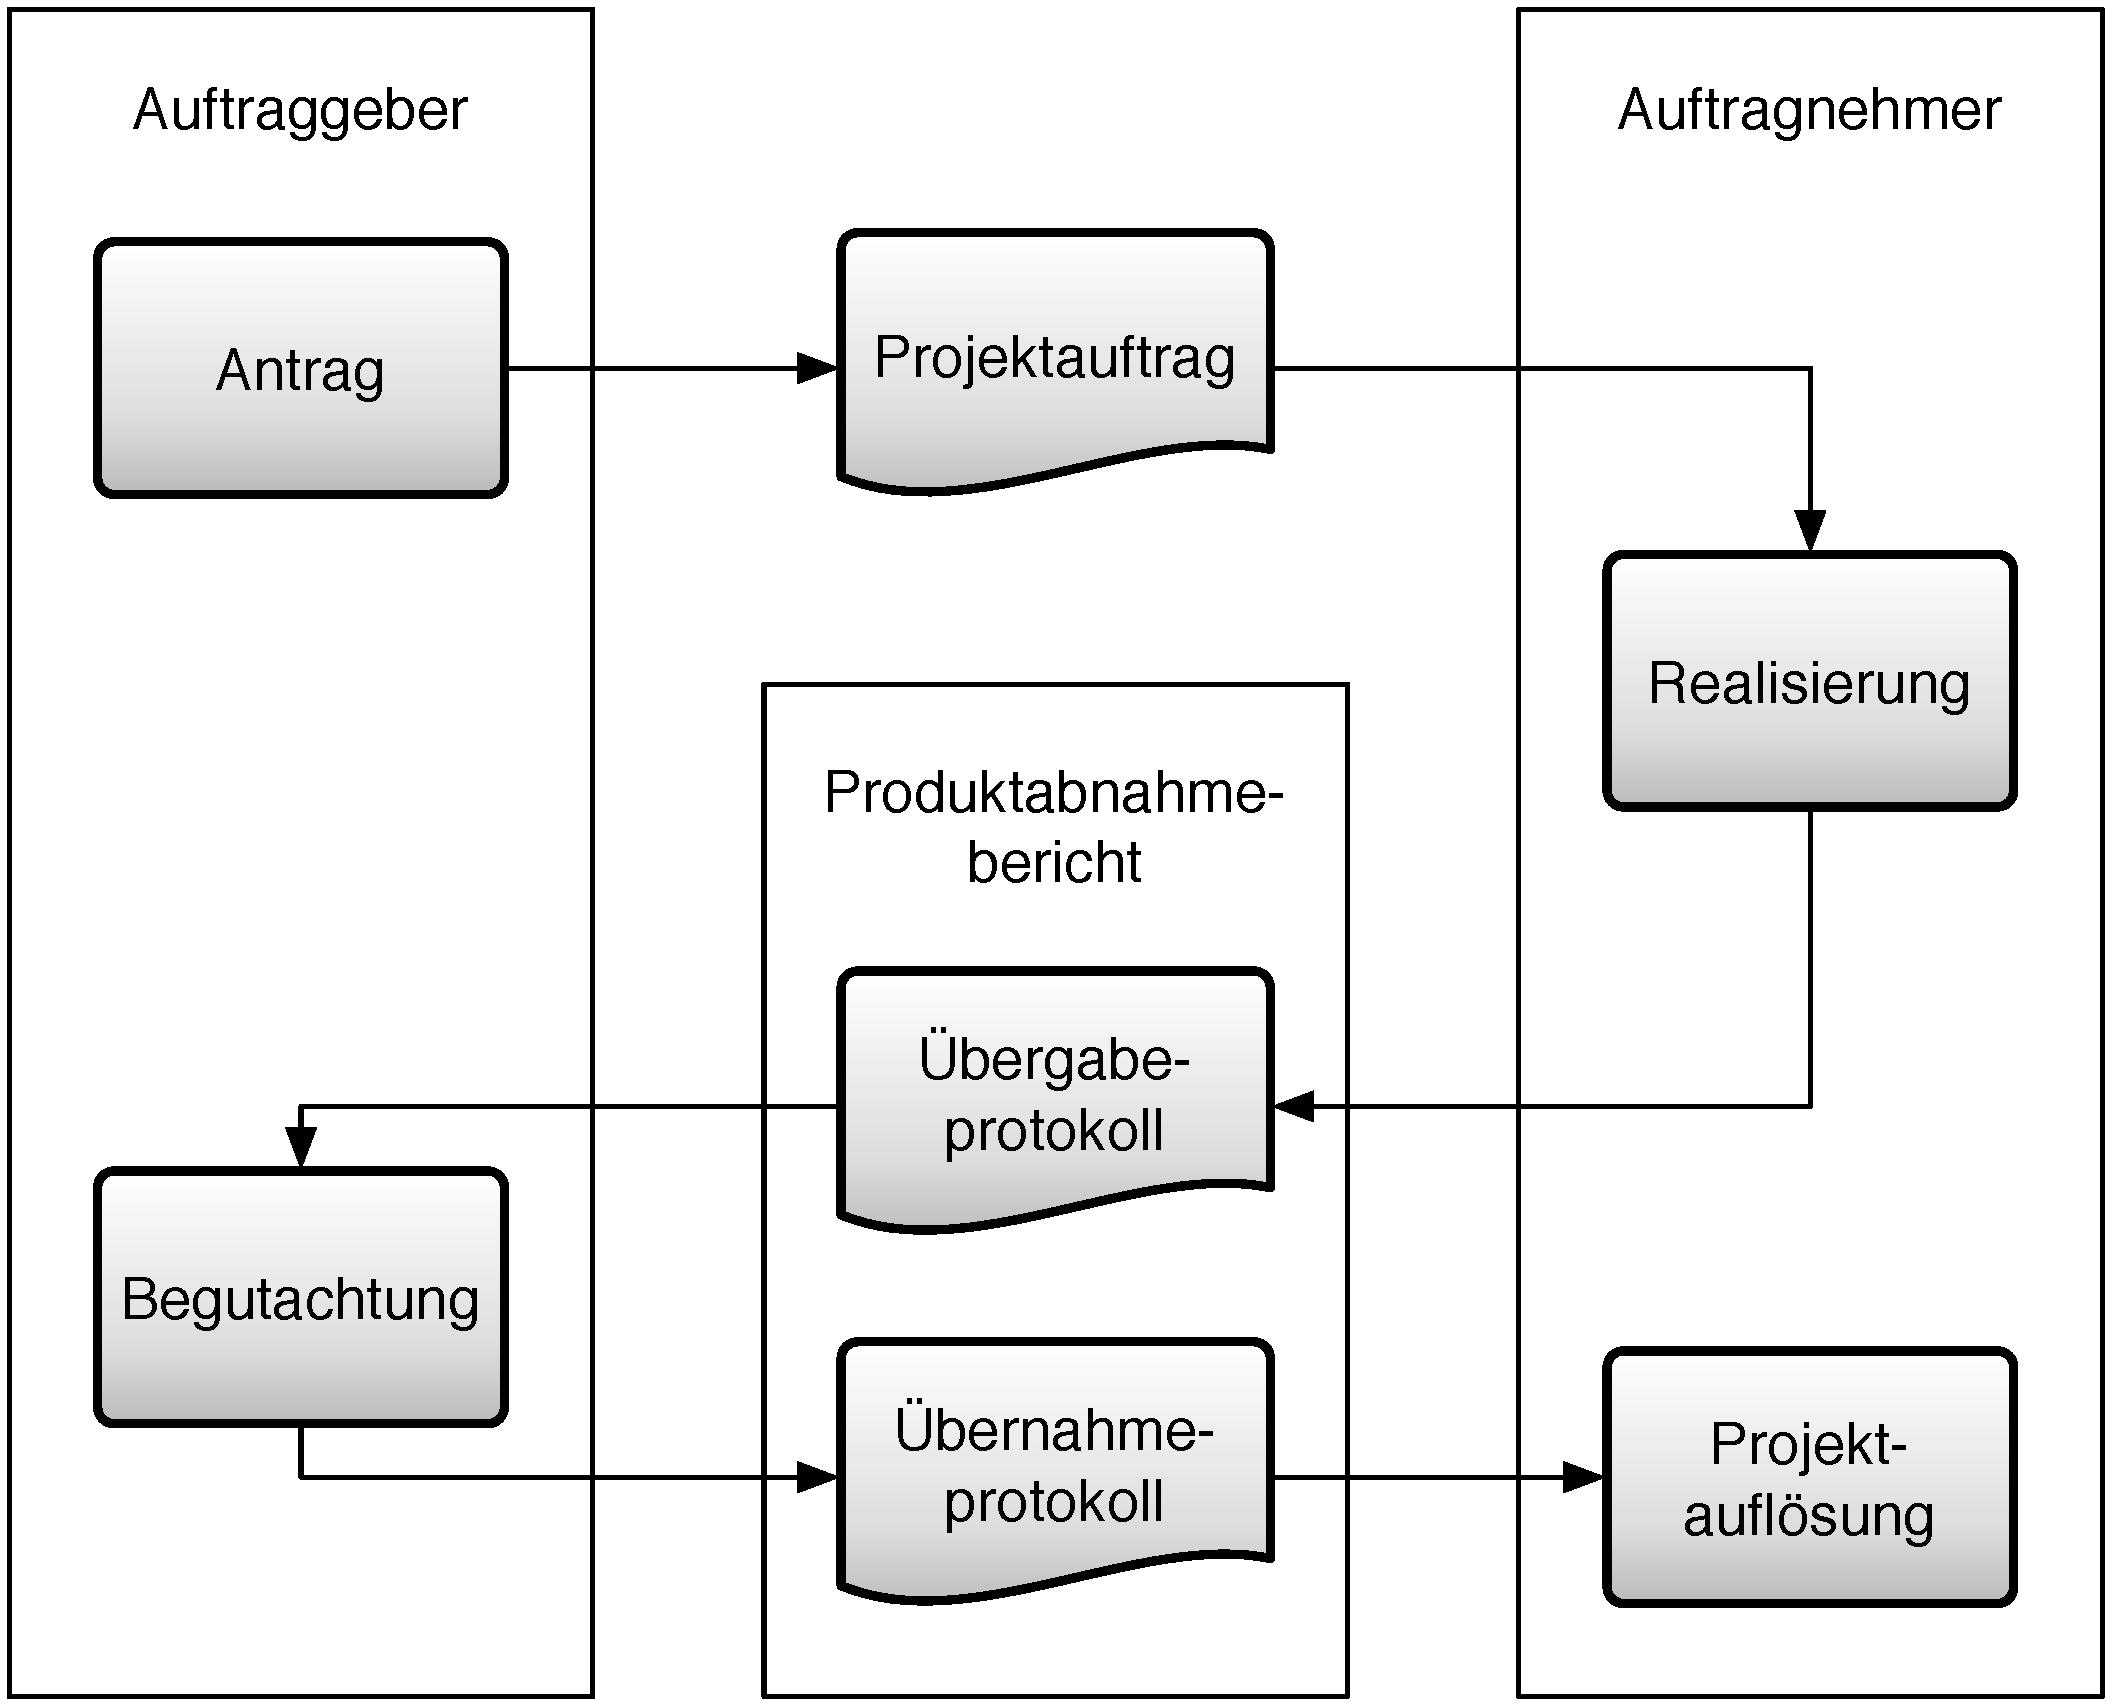
\includegraphics[width=0.6\textwidth,angle=0]{./bilder/theorie/07_produkteuebergabe.pdf}
\caption[Produkteabnahmebericht in der Produktübergabe]{Produkteabnahmebericht in der Produktübergabe\footnotemark}
\label{pic:07_produkteuebergabe}
\end{center}
\end{figure}
\footnotetext{Eigene Darstellung des Schemas in Anlehnung an \citealp*[Bild 5.2]{burghardt2007einfuehrung}}

Der Produktabnahmebericht sollte eine Beschreibung der Ergebnisse und eventuelle
Nachforderungen beinhalten. In der Regel beginnt nach der Abnahme die
Gewährleistungsfrist. Das bedeutet, dass der Zeitpunkt der Produktabnahme von
rechtlicher Relevanz sein kann und der Produktabnahmebericht vom Auftraggeber
unterschrieben werden sollte.\footnote{\citealp*[Vgl.][S. 86]{cronenbroeck2004handbuch}}
Zu diesem Zeitpunkt sollte man sich auch Gedanken über eine zukünftige Betreuung
machen.

In der Projektabschlussanalyse wird die ehemals erstellte Wirtschaftlichkeitsrechnung
auf ihre Einhaltung durchleuchtet. Zusätzlich werden die Einhaltung der Termine sowie
Leistungs- und Qualitätsmerkmale betrachtet. Wichtige Kennzahlen sind zudem
die Änderungshäufigkeit und Fehlerquote.\footnote{\citealp*[Vgl.][S. 265]{schelle2007projekte}}
Grundsätzlich sollten alle gesammelten Daten in eine Art Erfahrungsdatenbank 
des Unternehmens einfliessen. Diese stellen eine wichtige Voraussetzung für das 
Optimieren von Aufwandsschätzungen dar und können somit auf zukünftige Projekte 
eine positive Wirkung haben.\footnote{\citealp*[Vgl.][S. 275]{burghardt2007einfuehrung}}

\clearpage

\begin{figure}[htbp]
\begin{center}
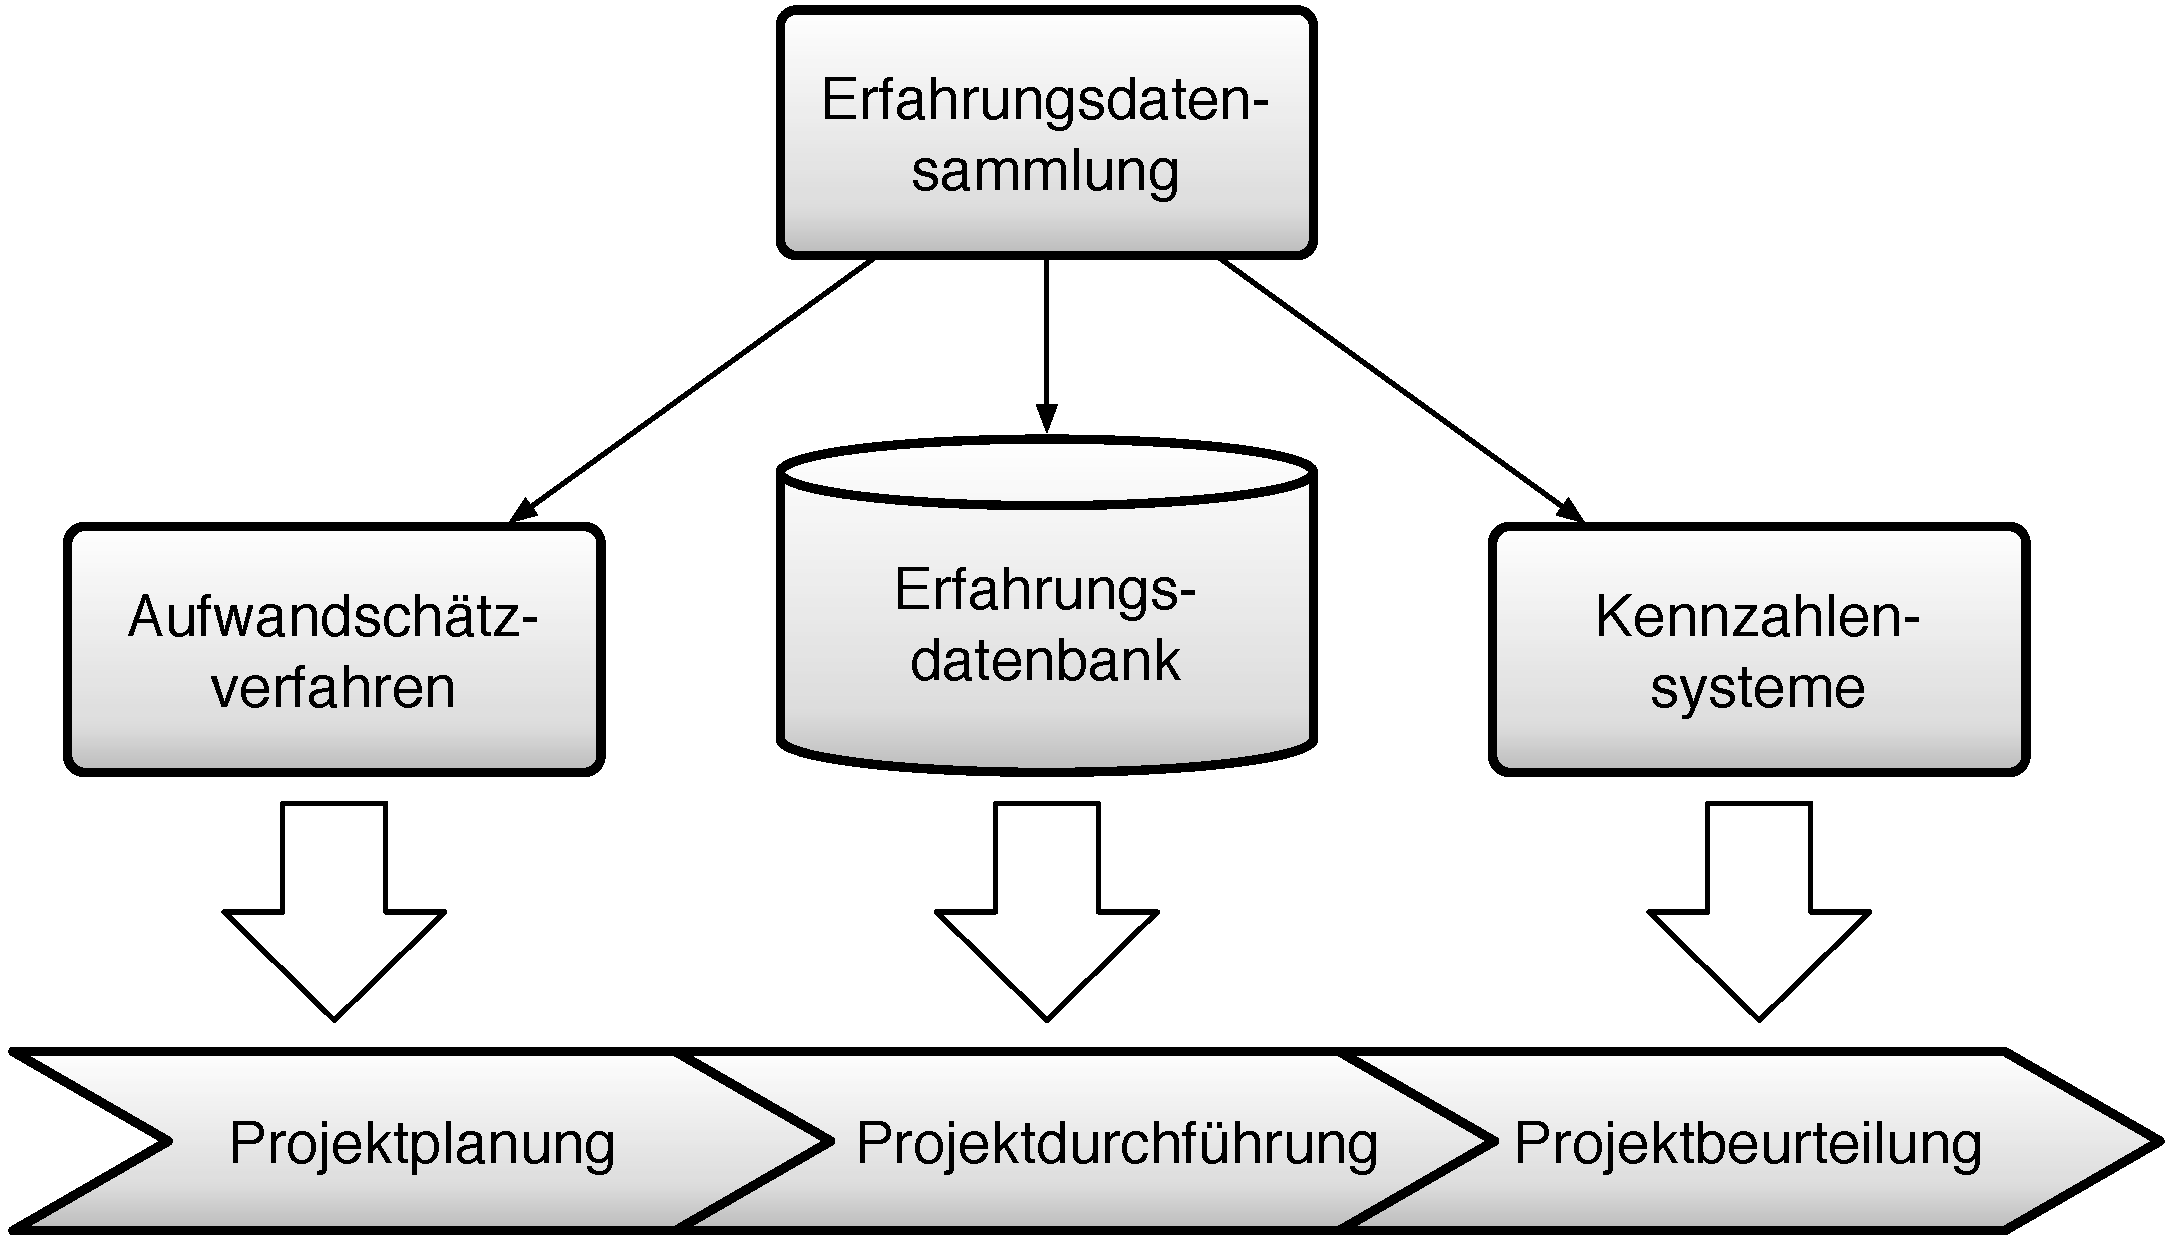
\includegraphics[width=0.6\textwidth,angle=0]{./bilder/theorie/04_unterteilung_erfahrungsdaten.pdf}
\caption[Unterteilung der Erfahrungsdaten]{Unterteilung der Erfahrungsdaten\footnotemark}
\label{pic:04_unterteilung_erfahrungsdaten}
\end{center}
\end{figure}
\footnotetext{Eigene Darstellung des Schemas in Anlehnung an \citealp*[Bild 5.7]{burghardt2007einfuehrung}}

Die Projektauflösung ist der letzte Schritt in der Projektabschlussphase. Wie 
zu Beginn erwähnt soll jedes Projekt auch ein eindeutiges Ende haben. Dies ist
für die Projektmitarbeiter besonders wichtig, da sie dann offiziell von dem
Projekt entbunden sind und in neue Projekte und Aufgaben übergeleitet werden
können. Möglicherweise ist es je nach Projekt auch sinnvoll, einen Abschluss
gebührend zu feiern.

\section{Zwischenfazit}
Die Theoretischen Grundlagen des Projektmanagements bieten einen guten Raster
mit genügend Flexibilität um einen Projektablauf auf verschieden Arten umzusetzen.
Es wird nun in der Analyse des bestehenden Projektablaufes im Kapitel \ref{chap:analyse}
darauf geachtet, welche Bereiche dieser Grundlagen bereits beachtet, umgesetzt
oder gar ganz ignoriert werden. An diesen Stellen wird jeweils auf die Theorie
verwiesen.

Bei der Aufnahme der Bedürfnisse und Anforderungen im Kapitel \ref{chap:anforderungen} 
wird darauf geachtet, welche Veränderungen bestrebt werden müssen um die in 
der Theorie empfohlenen Methoden und Hilfsmittel besser umsetzen zu können.
Beim zu erarbeitende Konzept im Kapitel \ref{chap:konzept} wird dann versucht, 
das neue Projektmanagement und den neuen Projektablauf stärker an die Theorie 
anzulehnen.